\chapter{Metode}
\textit{I dette kapitel beskrives de metoder som er anvendt til udvikling af en algoritme til kategorisering af  lægemiddelskift.}

\section{Udviklingstrin}
I udviklingsprocssen gennem gås forskellige step hvilket fremgår af Figur \ref{fig:XXX}

\begin{figure}[H]\centering	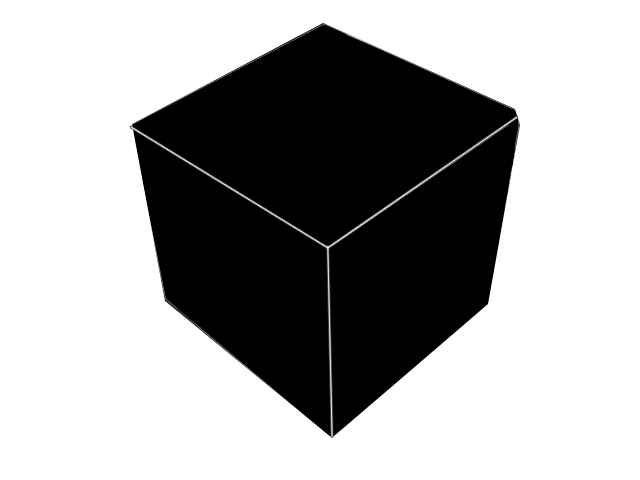
\includegraphics[width=0.5\textwidth]{billeder/Black_box.png} 
	\caption{XXXX.}
	\label{fig:XXX}  
\end{figure}

\section{Dataindsamling}
Indsamlet data omhandler Amgrosskift i år 2017. Disse data er enten indsamlet af Amgros eller af Sygehusapoteket Region Nordjylland (SRN) i forbindelse med lægemiddelskift. Data fra Amgros omfatter Amgrosskift fra år 2018 (Amgros2018)~\fxnote{Jeg har brug for at få data fra 2017 i stedet, da dette passer til det andet excel eller så skal jeg have et opdateret med amgrosskift i år 2018}. Data fra SRN omfatter amgrosskift fra år 2017\fxnote{OBS!} (SRN2018) og problemstillinger vedrørende amgrosskift (Problem), som omfatter dokumenteret problemstillinger fra år 2012 til 2017. Alt data er indsamlet i excelark, den opsamlede data kan ses af \ref{table:XXX}

\vspace{2mm}
\begin{longtable}{p{2.5cm}|p{1cm}|p{11cm}}
	\caption{**DET HER ER KUN TIL MIG SELV**}
	\vspace{2mm}
	\label{table:XXX} \\
\cellcolor[HTML]{C0C0C0} {\textbf{Data}} & {\cellcolor[HTML]{C0C0C0}\textbf{Antal}} & 
{\cellcolor[HTML]{C0C0C0}\textbf{Indhold}} \\ \hline
Amgros & 245 & Kontrakt start, ATC-kode, Varenummer 2017, Lægemiddel 2017, Dispenseringsform 2017, Styrke 2017, Pakningsstørrelse 2017, Varenummer 2018, Lægemiddel 2018, Dispenseringsform 2018, Styrke 2018, Pakningsstørrelse 2017, Bemærkning, Rekommenderet.\\ \hline
SRN & 5397 & ATC-koder, Matchstatus, Generisk navn, Firma, Varenummer, Forv. Varenummer, SA-Gl.Vnr (Kig Amgros estimering), Varenummerskift – 1 er skift 0 fortsætter (Kig Amgros estimering), Varenavn, Disponeringsform, Styrke, Pakning, Udbudsgruppe, Udbudsnummer (1-730), Vinder (1, 2, 3, 4, 5, 1x, 2x, BA, k), RADS-MR (0, 1) (RADS- medicin rådet måske medicinrådet??), Amg. Est., Budget pakning, Rev. Pakning, Bemærkning, SAIP/Pakning, AIP/Pakning,
AIP/Enhed, Enh./Paking , Budget slut, Indkøb start, Indkøb slut, Leadtime, Ingen prisvisning, Modified, ID, Created.\\ \hline
Problem & 103 & ATC-kode, Generisk navn, Firma, Varenummer, Varenavn, Udbudsgruppe, Udbudsnummer, Vinder, Debitor, Problemstilling/Bemærkning, Konsekvens, Simpel SAID-sag oprettet, Udfyldt af, Dato. \\ \hline
\end{longtable}



\section{Metode baggrund}
Der er to typer af mashine learning herunder unsupervised og supervised, da input-output relationer er kendt anvendes supervised machine learning. Inden for supervised learning anvendes kategorisering eller regression. Kategorisering identificerer en ny observation til et sæt af kategorier på baggrund af et træningssæt af data, hvor outputtet er kendt. Et eksempel på dette kan være at tildele en diagnose til en given patient baseret på patientens observerede egenskaber som f.eks. køn, blodtryk, tilstedeværelse eller fravær af visse symptomer. 

De enkelte observationer er ofte analyseret i et sæt kvantificerbare egenskaber, som er kendt forskelligt som forklarende variabler. Disse variabler kan have forskellige kategorier f.eks. stor, medium eller lille. Det kan også være antallet af forekomster af et  bestem ord. Andre klassifikationer arbejder med at sammenligne observationer til tidligere observationer ved brug af lighed og afstandsfunktioner.

En algoritme med disse egenskaber betegnes som en klassifikator, som henviser til den matematiske funktion, implementeret af en klassifikationsalgoritme, som kortlægger input til en kategori.

I maskinlæring er observationerne ofte kendt som forekomster, de forklarende variabler betegnes funktioner (grupperet i en funktionsvektor), og de mulige kategorier, der skal forudsiges, er klasser. 

\section{Regel-baseret system}
Tænkning i fakta og regler er måske en af ​​de mest almindelige måder at nærme sig problem definition og problemløsning både i hverdagen
liv og under mere formelle omstændigheder.
Det ønskes at udarbejde et regel-baseret system som kan gemme og manipulere viden til at fortolke information på en nyttig måde. Er adopteret fra artificial intelligence (AI) og knowledge engineering (KE). Regel-baseret systemer er sæt af regler, der efterligner logiske konsekvenser. Regel-baserede systemet udgør et kraftfuldt værktøj til specifikation af viden inden for design og implementering af vidensbaserede systemer (KBS) inden for anvendt kunstig intelligens og vidensteknik. 

Logiske regler
er dem defineret af mennesket; de er normalt subjektive, lokale, kan ændres
Hvis det er nødvendigt. Selvom regelbaserede systemer er et værktøj allestedsnærværende inden for videnskab, teknologi
og hverdagen er deres kodning, analyse og design sjældent et spørgsmål om
dybere teoretisk undersøgelse I de fleste af applikationsområderne bruges de netop (bevidst eller ubevidst) på en retfærdig måde, anvendt til at løse specifikt problem uden at være opmærksom på spørgsmål som deres egenskaber,
sprog, optimering osv. Selvom regelbaseret indledning ikke er
Den eneste mulighed for argumentation, logiske systemer er for det meste konstrueret som
sammensat af aksiomer (fakta) og indledning regler.

RBS til kontrol eller beslutningsstøtte
består af et enkeltlags sæt regler og en simpel inference-motor; det virker ved
Valg og udførelse af en enkelt regel ad gangen, forudsat at forudsætningerne
af reglen er opfyldt i den nuværende tilstand. 
At sikre pålidelighed, sikkerhed, kvalitet og effektivitet i regelbaserede systemer kræver både teoretisk indsigt
og udvikling af praktiske værktøjer. De generelle kvalitative egenskaber er
oversat til en række mere detaljerede egenskaber defineret i form af
logiske forhold.

For at opnå et rimeligt niveau af effektivitet (videnskabens kvalitet)
regelsættet skal udformes på en passende måde. Flere teoretiske
Egenskaber ved regelbaserede systemer synes at være værd at undersøge, begge
at give en dybere teoretisk indsigt i forståelsen af ​​deres kapacitet
og forsikre deres tilfredsstillende ydeevne, f.eks. pålidelighed og kvalitet. Nogle mest typiske spørgsmål om teoretisk verifikation
inkludere tilfredshed med egenskaber som konsistens, fuldstændighed, determinisme,
redundans, subsumption mv. (se [3, 81, 101]).

Men selv om teknologien i RBS bliver
mere og mere bredt anvendt i praksis på grund af dets forhold til første orden
logik og undertiden komplekse regelmønstre og inferencesystemer, de er stadig ikke godt accepteret af industrielle ingeniører.Desuden er den 'korrekte' brug af dem kræver meget intuition og domæneoplevelse og vidensamfund
udgør stadig en flaskehals for mange potentielle anvendelser.

I modsætning til RBS, Relational Data Base Systems (RDBS) [23, 30, 38, 131]
tilbyder relativt enkel, men modnet dataprofileringsteknologi, der anvender
bredt accepteret, intuitiv vidensrepræsentation i tabelform. Det ser ud til
fordelagtigt at gøre brug af elementer af denne teknologi til at forenkle visse
operationer vedrørende RBS.


%Anvendelse af regel-baseret systemer til vidensspecifikation og udvikling af praktiske applikationer er udbredt. Regel-baseret systemer anvender første orden logik, komplekse regel-mønstre og initiativer, hvilket gør at disse systemer kræver meget intuition og domæne erfaring for korrekt brug af systemet. Reglerne er baseret ud fra følgende princip:
%\vspace{-5mm}
%\begin{equation}
%Regel: Foruds\text{æ}tninger \rightarrow Konklusioner 
%\end{equation}
%Forudsætninger indeholder en formel, som definere hvornår regelen skal anvendes. Konklusioner definere effekten af at anvende reglen, herunder logisk attribut formel. 
%
%\begin{figure}[H]\centering	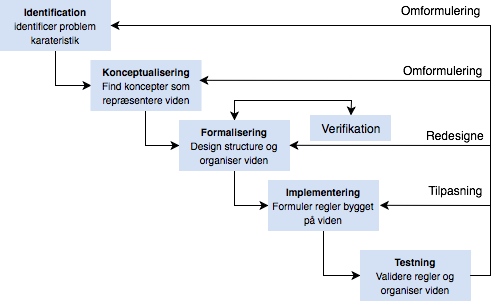
\includegraphics[width=1\textwidth]{Statusseminar/metode.png} 
%	\caption{XXXX.}
%	\label{fig:metode}  
%\end{figure}
%
%
%Da input-output relationen allerede er kendt anvendes supervised machine learning. Da formålet er at identificere hvilken kategori en ny observation tilhører anvendes klassificering.  

%
%\section{Data forberedelse} / Model
%- segmentation
%- farvetransformation - text/tal
%
%\section{Klassifikation}
%\subsection{Machine learning}
%\subsection{Feature for klassificering}
%\subsection{Neurale netværk som klassificering}
%
%\section{Validering}
%- klassificering performance matrics 
%
%
%dataindsamling
%data processering 
%feature extraction 